
\subsection{Árboles de decisión}

Este modelo tiene la ventaja de ser muy rápido pero presenta el problema de que si se deja crecer mucho el árbol el clasificador puede overfitear los datos de entrenamiento. Las primeras pruebas estuvieron orientadas estimar un rango de alturas en donde el clasificador tenga buena eficacia sin overfitear. Para lograrlo calculamos la métrica  f0.5 de arboles de alturas de 1 a 30 para datos de entrenamiento y para cross validation con K=10. En la figura ~\ref{fig:arboles_f05_en_funcion_altura} puede ver un gráfico de los resultados.

\begin{figure}[H]
    \centering
        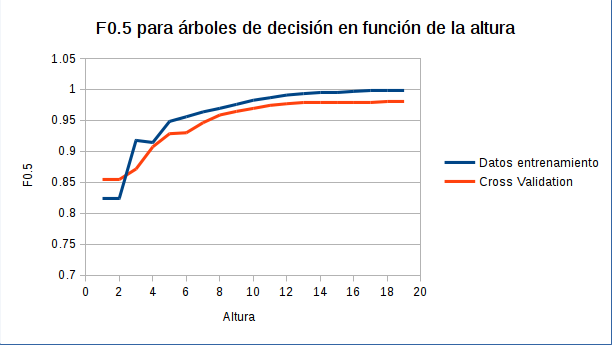
\includegraphics[width=\textwidth]{plots/arboles_f05_en_funcion_altura.png}
        \caption{f0.5 en funcíon de altura de árbol}
        \label{fig:arboles_f05_en_funcion_altura}
\end{figure}

	El resultado de cross validation es un estimador de la eficiencia que vamos a obtener clasificando correos nuevos y a pesar de que por lo general no aproxime correctamente la eficiencia nos permite predecir que estamos haciendo overfitting de datos de entrenamiento cuando al aumentar la altura baja o se mantiene la eficiencia. Como se puede ver en la figura ~\ref{fig:arboles_f05_en_funcion_altura} a partir de arboles de altura 9 el aumento en la eficacia al variar la altura especia a bajar hasta que se estanca llegando a arboles de altura 15. 
    Luego para para este rango de alturas ejecutamos un grid search a fin de obtener los mejores hiper-parametros para el clasificador. 
 \begin{enumerate}
\item \textit{criterio de selección:} Se probaron criterios, gini y ganancia de información. No se observaron grandes diferencias en la eficacia del clasificador al variar el criterio. El mejor resultado se obtuvo con ganancia de información. 
\item \textit{Cantidad máxima de atributos considerados:} Este hiper-parámetro permite limitar la cantidad de atributos considerados al hacer un split.  Tiende a favorecer al aparición de arboles que no sean dominados por los atributos que provean mayor ganancia de información, dado que es posible que varios atributos más débiles trabajando en conjunto logren mejor eficacia.  En las pruebas realizadas se obtuvieron mejores resultados sin limitar la cantidad de atributos
\item \textit{Cantidad mínima de elementos en división:} Limita la división de nodos internos a lo que superen en cantidad de elementos la cantidad especificada. Los mejores resultados se obtuvieron con el valor mínimo de 2. Al aumentar el valor y al mismo tiempo limitar las cantidad de atributos limitados se puede observar una caída de eficiencia en cross validation. 
\item \textit{Cantidad mínima de elementos en hojas:} Las hojas del árbol no pueden tener menos de la cantidad especificada. Los mejores resultados se obtuvieron con el valor mínimo de 2. Al igual que con el hiper-parámetro anterior, aumentar el valor y al mismo tiempo limitar las cantidad de atributos limitados se puede observar una caída de eficiencia en cross validation.  

\subsection{K-vecinos mas cercanos}

La idea de random forest es utlizar múltiples árboles de decisión para mejorar la eficacia del clasificador, reduciendo la alta varianza que se observa en la utilización de un único árbol. Esto es posible gracias al bajo costos que lleva entrenar y consultar a cada árbol. 
 La reducción en la varianza suele ser mas significativa cuando el bosque se arma con árboles que utilicen diferentes atributos. Para lograr esto los atributos utilizados en las divisiones de los nodo al construir el árbol se limitan a un subconjunto aleatorio de los atributos, reduciendo la probabilidad que lo atributos con mayor ganancia de información dominen todos los arboles. 
Utilizando los mismos parámetros que para el clasificador de un único árbol volvimos a hacer pruebas variando la cantidad de árboles del bosque y el tamaño del subconjunto de atributos a considerar. En la figura ~\ref{fig:forest_f05_en_funcion_de_cantidad_de_arboles} se muestran los resultados para bosques de diferentes tamaños considerando n, $\sqrt{n}$ y $\log(n)$ atributos, donde n es la cantidad total de atributos. Los bosques en loas cuales se consideran n atributos muestran mejores resultados, pero cuando consideran $\sqrt{n}$ atributos,  la varianza es inferior por lo que esperamos que la eficacia con datos nuevos sea más parecida a lo  que observamos con cross validation sobre datos de entrenamiento. 

\begin{figure}[H]
\begin{center}
\myss{0.45}{random_forest.pdf}{$f_{0.5}$ en funcíon de cantidad de árboles}{0.35}
\myss{0.45}{random_forest_var.pdf}{varianza enfuncíon de cantidad de árboles}{0.35}
\caption{Resultados grid search random forest}
\label{fig:forest_f05_en_funcion_de_cantidad_de_arboles}
\end{center}
\end{figure}
\subsection{Random Forest}

La idea de random forest es utlizar múltiples árboles de decisión para mejorar la eficacia del clasificador, reduciendo la alta varianza que se observa en la utilización de un único árbol. Esto es posible gracias al bajo costos que lleva entrenar y consultar a cada árbol. 
 La reducción en la varianza suele ser mas significativa cuando el bosque se arma con árboles que utilicen diferentes atributos. Para lograr esto los atributos utilizados en las divisiones de los nodo al construir el árbol se limitan a un subconjunto aleatorio de los atributos, reduciendo la probabilidad que lo atributos con mayor ganancia de información dominen todos los arboles. 
Utilizando los mismos parámetros que para el clasificador de un único árbol volvimos a hacer pruebas variando la cantidad de árboles del bosque y el tamaño del subconjunto de atributos a considerar. En la figura ~\ref{fig:forest_f05_en_funcion_de_cantidad_de_arboles} se muestran los resultados para bosques de diferentes tamaños considerando n, $\sqrt{n}$ y $\log(n)$ atributos, donde n es la cantidad total de atributos. Los bosques en loas cuales se consideran n atributos muestran mejores resultados, pero cuando consideran $\sqrt{n}$ atributos,  la varianza es inferior por lo que esperamos que la eficacia con datos nuevos sea más parecida a lo  que observamos con cross validation sobre datos de entrenamiento. 

\begin{figure}[H]
\begin{center}
\myss{0.45}{random_forest.pdf}{$f_{0.5}$ en funcíon de cantidad de árboles}{0.35}
\myss{0.45}{random_forest_var.pdf}{varianza enfuncíon de cantidad de árboles}{0.35}
\caption{Resultados grid search random forest}
\label{fig:forest_f05_en_funcion_de_cantidad_de_arboles}
\end{center}
\end{figure}
\end{enumerate}
